\begin{figure*}[!htb]
\minipage{0.22\textwidth}
  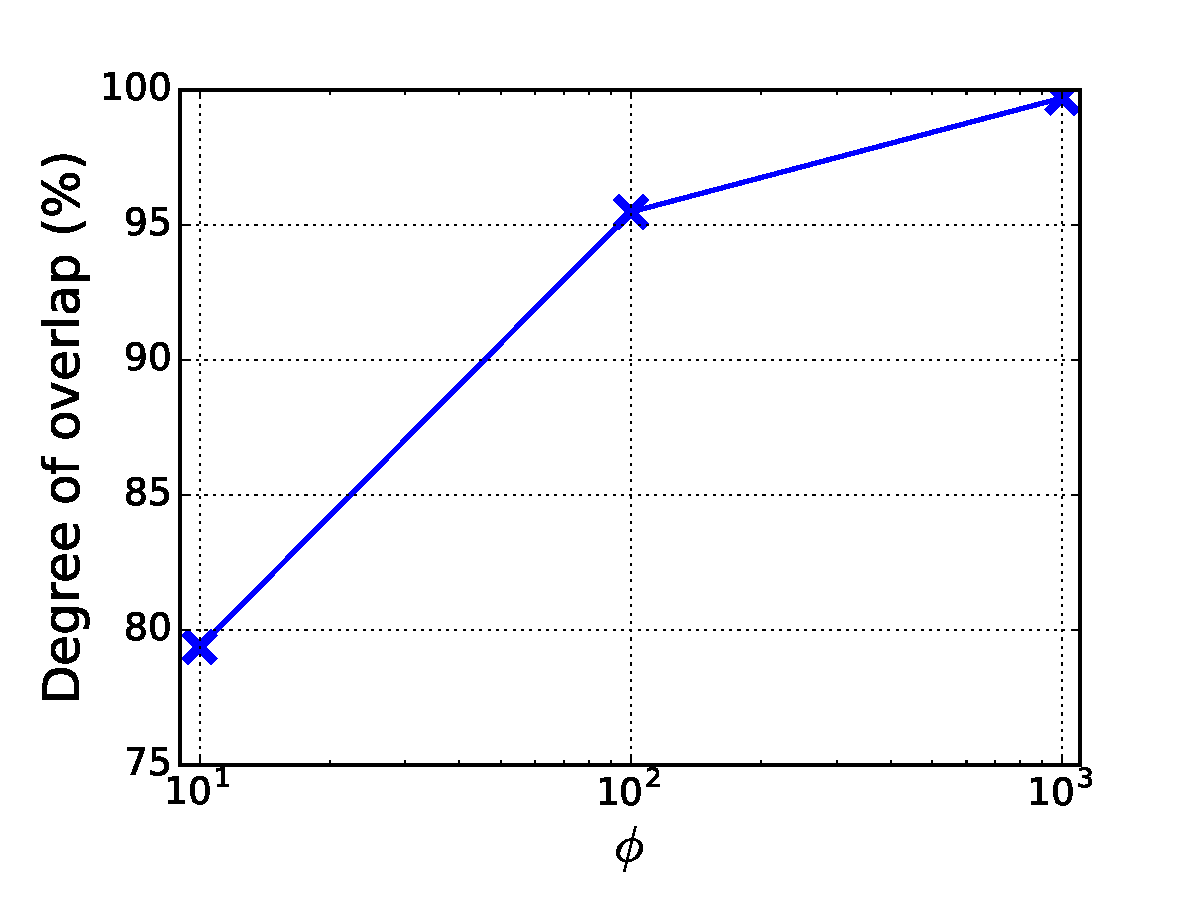
\includegraphics[width=\linewidth]{figure/overlap.pdf}
  \mycaption{fig:overlap}{Relation between $\phi$ and degree of overlap.}
  {How the degree of overlap changes with the change of $\phi$ from $10^1$ to $10^3$.}
  %\label{fig:overlap}
\endminipage\hfill
\minipage{0.22\textwidth}
  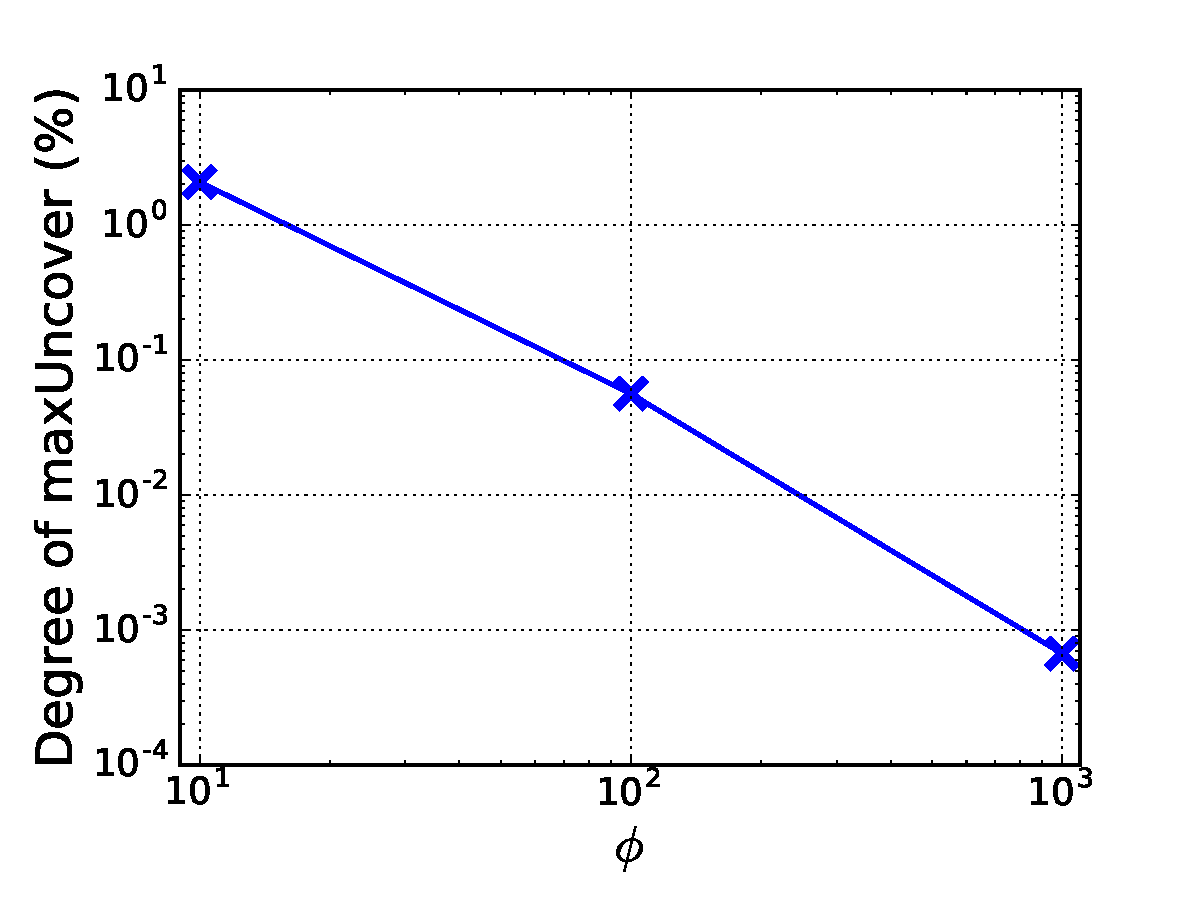
\includegraphics[width=\linewidth]{figure/maxUncover.pdf}
  \mycaption{fig:maxUncover}{Relation between $\phi$ and degree of maxUncover.}
  {How the degree of maxUncover changes with the change of $\phi$ from $10^1$ to $10^3$.}
  %\label{fig:maxUncover}
\endminipage\hfill
\minipage{0.22\textwidth}%
  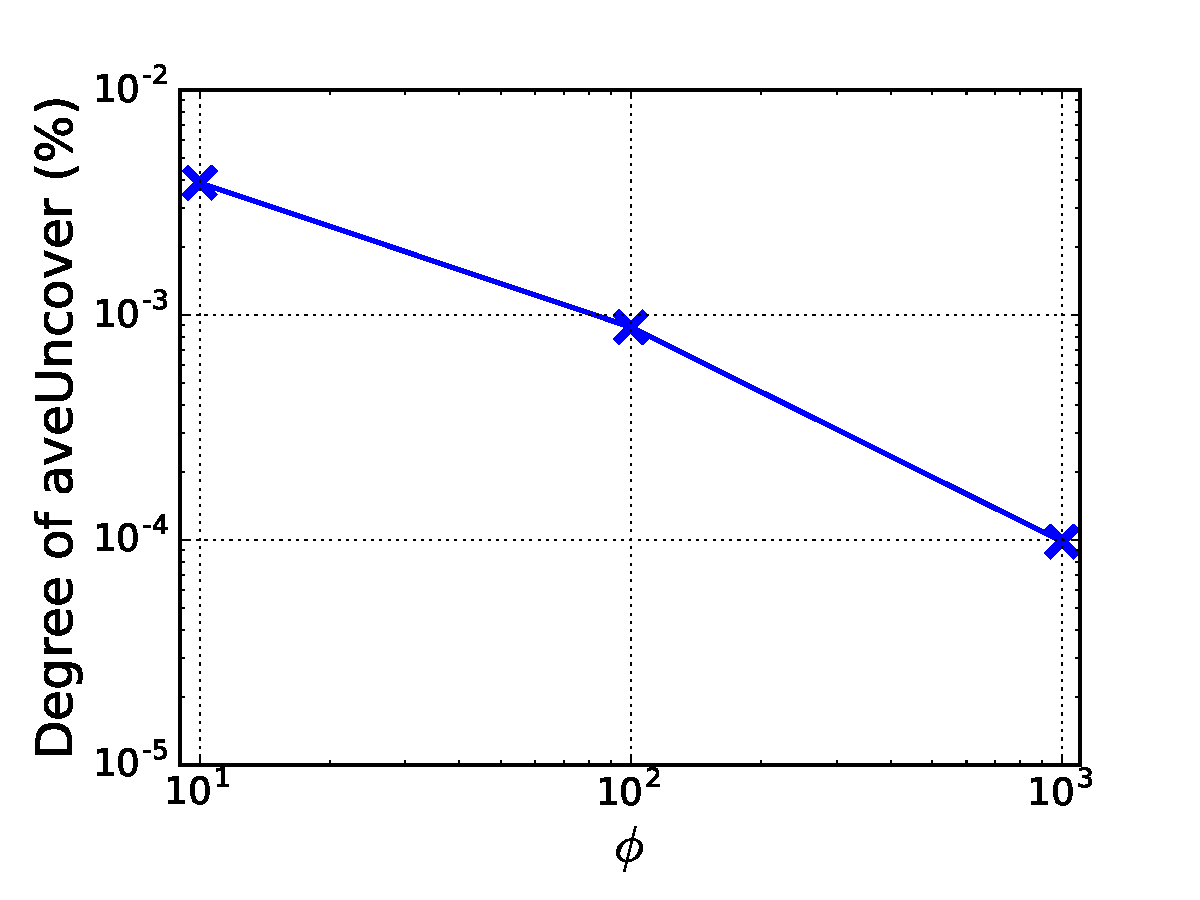
\includegraphics[width=\linewidth]{figure/aveUncover.pdf}
  \mycaption{fig:aveUncover}{Relation between $\phi$ and degree of aveUncover.}
  {How the degree of aveUncover changes with the change of $\phi$ from $10^1$ to $10^3$.}
  %\label{fig:aveUncover}
\endminipage\hfill
\minipage{0.22\textwidth}%
  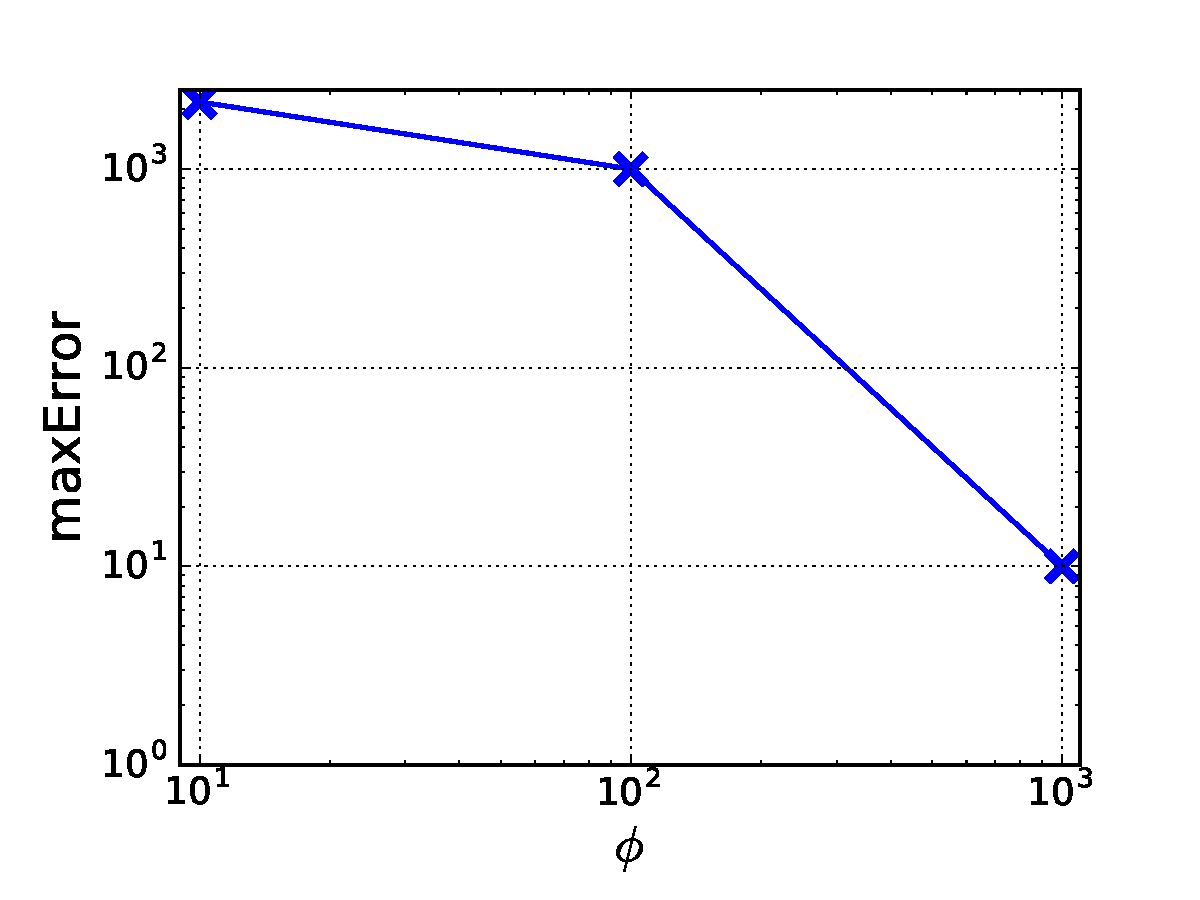
\includegraphics[width=\linewidth]{figure/maxError.pdf}
  \mycaption{fig:maxError}{Relation between $\phi$ and maxError.}
  {How maxError changes with the change of $\phi$ from $10^1$ to $10^3$.}
  %\caption{Relation between $\phi$ and maxError.}
  %\label{fig:maxError}

\endminipage
\vspace{-0.1in}
\end{figure*}